\documentclass[preprint,linenumbers, longauthor]{aastex631}
\bibliographystyle{aasjournal}
\usepackage{graphicx}
\usepackage{appendix}
\usepackage{listings} 
\usepackage{xcolor}
\usepackage{amsmath}
\begin{document}

\title{The New Age of Big Data In Astronomy: A Review of the SKA \& Rubin}
\author{Mathew Icho}
\affiliation{The University of Illinois at Urbana-Champaign}

\begin{abstract}
I'm making my abstract my to do list for now

\textbf{2. Find a paper or part of it that describes how SDSS stores the data. I don't think I've dont that sufficiently}

\textbf{3. Do the LSST part}

\textbf{4. Do the Results section, look at data collected. I plan on coding A LOT for this section}

\end{abstract}

\tableofcontents

\section{Introduction}
%Start with kind of a summarized overview with the paper
%Then go to history of data being handled in Astronomy
%Then go talk about Moore's law%Then talk about main idea of this paper, say how its gonna be structured
The concept of data has long been central throughout the history of astronomy. Data allows scientists to discover natural laws in the universe, have control over events, and make reliable predictions. It has played a critical role in other time-sensitive fields such as medicine and engineering, where accurate data is essential for decision-making and design. 
Although the nature of data varies fundamentally across different fields, one trend has remained consistent: the continual evolution of data science. As explained in The Fourth Paradigm \citep{heyFourthParadigmDataIntensive2009}, this evolution can be characterized through four successive paradigms. 
In the following sections, I describe the progression of data acquisition across these paradigms and illustrate each using examples from astronomy. I will then explain how SKA and LSST fit into this trajectory and exemplify the emerging era of data-intensive discovery.
\subsection{The Paradigms of Data Science}
The first and most primitive paradigm, as described by \citep{heyFourthParadigmDataIntensive2009}, is empirical evidence. 
Empirical evidence refers to data collected through traditional means, such as direct observation or experimentation. 
The primary purpose of empirical evidence is to identify patterns that allow scientists to develop a fundamental understanding of the natural world. 
Throughout much of human history, empirical evidence has dominated knowledge generation. 
An example of the first paradigm in astronomy is the career of Tycho Brahe, a Danish astronomer. Throughout his career in the 16th century, Brahe collected and cataloged data on the position of astronomical bodies using naked-eye observations. Tycho Brahe's catalogue was accurate to only around 1' precision and took decades to acquire \citep{verbuntThreeEditionsStar2010}.
However, empirical evidence can be compromised by human error, the precision of the instruments, and, most importantly, the relatively slow pace of data acquisition compared to subsequent paradigms.

The second paradigm is analytical evidence. Analytical evidence is obtained by constructing mathematical formulas and theoretical frameworks based on empirical data \citep{heyFourthParadigmDataIntensive2009}. 
Unlike the empirical evidence, which merely demonstrates that phenomena occur, the second paradigm seeks to explain why they occur. 
An example of the second paradigm in astronomy is the work of Johannes Kepler, who used Brahe's empirical observations to derive the laws of planetary motion \citep{heyFourthParadigmDataIntensive2009}. 
By transforming raw observational data into mathematical laws, Kepler exemplified how analytical evidence advances scientific understanding beyond description to explanation.

The third paradigm is simulation evidence \citep{heyFourthParadigmDataIntensive2009}, a relatively recent development. Simulation models natural phenomena that are too complex to model analytically or compute by hand. 
It allows interpolation and extrapolation of data using computational techniques grounded in known physical laws. 
For example, in astronomy, N-body simulations are used to study the complex dynamical evolution of planetary systems and galaxies. 

The fourth and most recent paradigm is data-intensive science \citep{heyFourthParadigmDataIntensive2009}. 
This paradigm is characterized by the unprecedented scale, velocity, and complexity of data acquisition, driven in part by exponential advances in computational power and detector technologies, often associated with Moore's law \citep{heyFourthParadigmDataIntensive2009}. 
Unlike earlier paradigms, which focused on observation, theory, or simulation, data-intensive science emphasizes the ability to manage, analyze, and interpret vast datasets that exceed the capacity of traditional methods. 
While this exponential growth in data has enabled transformative discoveries, it also introduces significant challenges related to storage, processing, and accessibility. 

\subsection{The Rise of Big Data in Astronomy}
Astronomy has become data intensive. Modern observatories may now generate petabyte-scale data that need new strategies for data management and analysis \citep{heyFourthParadigmDataIntensive2009}. 
The fourth paradigm enables discoveries from interpreting massive data sets. 
However, these advances also expose alarming issues, including bottlenecks in the data pipeline, storage challenges, increased skills needed to handle the data, and open access concerns. 
The field of astronomy is both a beneficiary and a victim of this data-intensive transition. 

As mentioned above, the exponential growth of data acquisition can be attributed to Moore's law \citep{heyFourthParadigmDataIntensive2009}.  
Moore's law predicts that integrated circuit chip density doubles approximately each year at a fixed price point \citep{mooreCrammingMoreComponents2006}.
\citep{mooreCrammingMoreComponents2006} questioned whether technical development would sustain the growth.

Moore's law can be seen in many data-intensive fields, including astronomy.
It explains both the recent development of big data in astronomy, and predicts future challenges.

This paper therefore seeks to review the rise of big data in astronomy and the technical and scientific issues surrounding it by examining four case studies: MeerKAT \footnote{\url{https://www.skao.int/en}}, The Sloan Digital Sky Survey (SDSS) \footnote{\url{https://www.sdss.org/}}, The Legacy Survey of Space and Time (LSST) \footnote{\url{https://www.lsst.org/}}, and The Square Kilometre Array (SKA) \footnote{\url{https://www.skao.int/en}}. 
These facilities represent the scope of contemporary astronomical data, the methods of its acquisition, their relative successes, the ongoing challenges, and the solutions currently in use.

\subsection{An Overview of The Four Surveys}
The SDSS is vital to this paper, as it is one of the earliest large-scale optical surveys that marks the start of the fourth paradigm. 
The SDSS is a precursor to LSST. The SDSS
consists of three main telescopes.

The first of the three is The Sloan Foundation 2.5m Telescope. 
The Telescope is stationed at the Apache Point Observatory in New Mexico, where it observes the sky in the northern hemisphere. 
It is able to observe a 3$^\circ$ field of view by use of two corrector lenses \citep{gunn25TelescopeSloan2006}.

The SDSS also uses the Irénée du Pont telescope at Las Campanas Observatory \footnote{\url{https://www.lco.cl/irenee-du-pont-telescope/}}. This telescope is stationed in Chile, where it observes the southern hemisphere instead. 
Similar to the foundational telescope at Apache Point, this telescope has a 2.1$^\circ$ field of view but only uses one corrector lens \citep{bowenOpticalDesign40in1973}.

The third telescope is the NMSU 1-meter Telescope \footnote{\url{https://newapo.apo.nmsu.edu/}}. The NMSU telescope is stationed at the Apache Point Observatory alongside the foundational telescope. 
The NMSU telescope is designed to observe bright stars that are too bright for the aforementioned two telescopes to observe \citep{majewskiApachePointObservatory2017}. 

the SDSS is made up of multiple subsurveys. The eBoss survey \footnote{\url{https://www.sdss4.org/surveys/eboss/}}, a continuation of BOSS, uses spectrographs to observe light in a wavelength range of 3600-10,400~\AA \space \citep{dawsonSDSSIVEXTENDEDBARYON2016}.
An additional subsurvey is APOGEE-2, a continuation of APOGEE. It uses spectrographs similar to eBOSS, but APOGEE-2 collected near-infrared spectra \citep{majewskiApachePointObservatory2017}. 
MaNGA \footnote{\url{https://www.sdss4.org/surveys/manga/}} is a subsurvey that collects integral field unit spectra of 10,000 nearby galaxies \citep{bundyOVERVIEWSDSSIVMaNGA2014}.
MARVELS \footnote{\url{https://www.sdss4.org/surveys/marvels/}} is another SDSS subsurvey, it was built specifically to obtain radial velocity measurements of stars with high-precision in hopes of finding exoplanets \citep{bundyOVERVIEWSDSSIVMaNGA2014a}.


The MeerKAT \footnote{\url{https://www.sarao.ac.za/science/meerkat/}} is an important precursor telescope to the SKA \citep{jonasMeerKATRadioTelescope2018}
MeerKAT became fully operational in 2018 in the Northern Cape Province of South Africa.
MeerKAT comprises 64 antennas distributed over a radius of approximately 600 miles \citep{goedhartMeerKATSpecifications2025}. These antennas operate across frequency bands ranging from 350 MHz to 3500 MHz \citep{goedhartMeerKATSpecifications2025}.

MeerKAT has conducted and continues to conduct ten major survey projects \citep{jonasMeerKATRadioTelescope2018}. For conciseness, this discussion will focus on five of these surveys.
One is the LADUMA \footnote{\url{https://science.uct.ac.za/laduma}} survey.
The objective of the LADUMA survey is to use HI obversations to research galaxy evolution over approximately 9.8 billion years \citep{blythLADUMALookingDistant2018}. 
LADUMA has used MeerKAT's Phase 1 receivers, which cover 0.9-1.75 GHz. It later transitioned to longer observations in Phase 4, which cover the 0.58-2.5 GHz band \citep{blythLADUMALookingDistant2018}.
Although the LADUMA survey is still ongoing, a portion of the data has already been released and will be discussed in the Methods section.

The MeerKAT absorbtion line survey \footnote{\url{https://mals.iucaa.in/}} (MALS) is a survey of HI and OH absorbers at a redshift of $z < 0.4$ and $z < 0.7$. 
HI is a descriptive tracer of the cold neutral medium in a galaxy \citep{guptaBlindOHAbsorption2021}. 
The cold neutral medium contains the physical conditions of the interstellar medium of each galaxy. This, in turn, allows scientists to estimate star formation rate in the galaxy \citep{guptaBlindOHAbsorption2021}.

Another survey, ThunderKAT \footnote{\url{https://www.physics.ox.ac.uk/research/group/meerkat}}, aims to find, identify and understand high-energy radio transients, usually grouped with observations at similar wavelengths.
Examples include supernovae, microquasars, and similar events \citep{woudtThunderKATMeerKATLarge2018}.

Another notable MeerKAT survey is MHONGOOSE \footnote{\url{https://mhongoose.astron.nl/}}. This survey aims to catalogue the properties of HI gas using 30 nearby star-forming spiral and dwarf galaxies. 
MHONGOOSE is remarkable for its higher sensitivity compared to previous surveys such as HALOGAS \footnote{\url{https://www.astron.nl/halogas/}} and THINGS \footnote{\url{https://www2.mpia-hd.mpg.de/THINGS/Overview.html}} \citep{deblokMHONGOOSEMeerKATNearby2024}. 
This sensitivity is crucial for investigating how low-column-density gas influences the cosmic web and galactic accretion processes \citep{deblokMHONGOOSEMeerKATNearby2024}.

The final MeerKAT survey considered here is MIGHTEE \footnote{\url{https://www.mighteesurvey.org/home}}. MIGHTEE spans 900-1670 MHz, achieving a resolution of approximately 6 arcseconds. MIGHTEE seeks to study the evolution of active galatic nuclei, neutral hydrogen, and the properties of cosmic magnetic fields \citep{MIGHTEESurvey}.

\begin{figure}[h!]
  \centering
  \includegraphics[width=0.8\textwidth]{SKA_Graph.png}
  \caption{Figure 3 from the SKA Official website \footnote{\url{https://www.skao.int/en/science-users/118/ska-telescope-specifications}}, SKA1 sensitivity compared to existing facilities at similar frequencies}
  \label{fig:SKA_Graph}
\end{figure}

The SKA has built on technical and scientific achievements paved by MeerKAT and other radio interferometers.
The SKA covers an area of approximately 131,205 antennas \citep{SKATelescopeSpecifications}. The SKA represents the start of a new frontier for big data in astronomy.
As an interferometer it uses aperture synthesis, which allows for the signals from antennas to be phased, this allows to reduce noise \citep{dewdneySquareKilometreArray2009}. The SKA will be discussed in further detail in the Methods section. 

Alongside the SKA is its optical big data counterpart, the LSST.
As noted above, the LSST is a successor to the SDSS. Rubin/LSST, however, has much more sophisticated goals. The LSST plans to address four key scientific issues:Investigating dark energy and dark matter, cataloguing the solar system, collecting data for sky surveys, and mapping the Milky Way.
To achieve this, the LSST uses a 3.2-gigapixel camera with a sampling of 9.6 deg$^2$ field of view \citep{ivezicLSSTScienceDrivers2019}. These cameras are equipped with highly resistant sensors reinforced with silicon \citep{ivezicLSSTScienceDrivers2019}. Rubin/LSST has an unprecented data rate for an optical telescope.

The SDSS, MeerKAT, SKA, and LSST generate unprecedented data rates and allow the experimentation of complex astrophysical events and phenomena.
In the following Methods section, I describe how the data are collected, processed, analyzed, and stored. I then compare SDSS and MeerKAT to their larger successor telescopes, Rubin/LSST and SKA and consider the evolution of data challenges.

\section{Methods}

%Methods:
%○ Approach to collecting Data
%● Talk about how the LSST and SKA are collecting data
%○ The nature of their data, ie the scope, type, etc
%■ LSST is optical imaging
%■ SKA is radio interferometry
%○ How they’re storing/archiving the data.
%○ How they’re generally processing their data
%○ Transparency of their respective Data pipeline
%○ Real time processing techniques (NOTE: NOT THE SAME AS THE METHODS
%DATA PROCESSING, THIS ONE IS FOR REAL TIME PROCESSING)
    %■ Show new techniques being developed to combat issues such as
    %optimization and time important issues

%LSST FIRST??
\subsection{The Optical Big Data Pipeline}

This section carefully examines how each of the optical focused surveys collects and processes its data. 
By describing the nature, scope, and type of the data. 
Next, we discuss how each survey collects and archives its data, followed by an explanation of their general data processing methods. 
Finally, we consider the use of real-time data processing. 
%By comparing these surveys, this study highlights the rapid growth of big data in astronomy, a trend that has created challenges for data storage, processing, and analysis. 
%These challenges will be discussed further in the discussion section.

As noted Above, we can consider the SDSS to consist of three main components: the 2.5 m foundational telescope, the Irénée du Pont telescope, and the NMSU 1-meter telescope.
The SDSS has evolved rapidly overtime. In the early 2000's the SDSS was primarily focused on optical imaging, but ever since the mid 2010's it has shifted towards gathering spectral data \citep{yorkSloanDigitalSky2000,ahumada16thDataRelease2020}
As discussed previously, we will consider how each telescope collects data, how the SDSS processes the data, and makes the data acessible through an open data policy.

\subsubsection{The Sloan Digital Sky Survey (SDSS)}
\paragraph{Data Collection and Storage} 

\textbf{(1) The SDSS 2.5 m Foundational Telescope:}  
The SDSS camera contains 54 2048 x 2048 charge-coupled devices (CCDs) and 24 2048 x 400 CCDs.
A CCD is an imaging detector that converts incoming light into an electronic signal. 
When photons strike the CCD, they generate electrons through the internal photoelectric effect. 
The acculumated charge is measured per pixel and is stored as a digital value \citep{lesserSummaryChargeCoupledDevices2015}.

In addition to the CCD imaging data the SDSS collects spectra using a pair of fiber-fed double spectrographs, over a wavelength range from 3800 to 9200~\AA\ and at field angles between 0 and 90$^{\circ}$ \citep{gunn25TelescopeSloan2006}. 
The spectrograph fibers are positioned in pre-selected objects of the field. The optical performance of these spectrographs, which are summarized in Table 5 from \cite{gunn25TelescopeSloan2006}.

\begin{figure}[h!]
  \centering
  \includegraphics[width=0.4\textwidth]{gunn_table_5.png}
  \caption{Figure 5 from Gunn et al. (2006), Telescope Optical Performance for the Spectrographic Mode: Average Focus}
  \label{fig:SDSS_Table}
\end{figure}

In Figure~5, $\lambda$ represents wavelength, and “Angle” refers to the field angle. 
$f_b$ denotes the best-focus distance. 
$h/dh$ represents the lateral color, $D$ denotes the longitudinal difference from the best focus, and $\epsilon$ is the root mean square (rms) image diameter. 
Smaller values of the lateral color and longitudinal difference indicate sharper images. 
Both of these quantities remain close to zero for most wavelengths and field angles, except between roughly 5300 and 6500~\AA \citep{gunn25TelescopeSloan2006}. This demonstrates the high optical accuracy of the SDSS spectrographs.
The 2.5 m telescope collects imaging and spectroscopic data at a rate of about 20Gb/hr \citep{luptonSDSSImagingPipelines2007}.

\textbf{(2) The Irénée du Pont Telescope:}  
The du Pont telescope data collection has evolved overtime \citep{bowenOpticalDesign40in1973}. It used to collect imaging data, which I will talk about first. 
In recent times, such as the 16th SDSS data release, the Du Pont telescope is used for collecting spectra data \citep{ahumada16thDataRelease2020}, which is what I'll talk about later.

During its optical era, the telescope is a modified Ritchey-Chrétien design with Gascoigne correcton and a 100-inch primary mirror \citep{bowenOpticalDesign40in1973}. Approximately 40\% of the light is reflected to the secondary mirror, resulting in only a 16\% loss of light at that stage. \citep{bowenOpticalDesign40in1973}

The du Pont Telescope used 18.9 inch nonvignetted plates in order to minimize vignetting \citep{bowenOpticalDesign40in1973}. Vignetting is the process where light beds through the lense of a telescope. The bending form a cone of light, which causes images to be darker near the edges and brighter in the center of the image \citep{richardsWhatVignetting2020}.
Because of the nonvignetted plates, the du Pont Telescope experiences an exceptionally low 3\% percent loss of light \citep{bowenOpticalDesign40in1973}.

Another technology the du Pont Telescope applied was a Gascoigne corrector plate. The plate helped with data collection. The Gasciogne corrector plate was abled to be moved, which could help optimize the collection of light in a wanted wavelength \citep{bowenOpticalDesign40in1973}.
Given a seperation of 1000 mm from the end of the corrector plate to the focus gave an image with a minimized astigmatism for a refractive index of n = 1.47 \citep{bowenOpticalDesign40in1973}.
At a given wavelength, the change of length which minimized astigmatism is described in Bowen's paper as

\begin{equation}
\Delta L = 590\Delta n / (n - 1) = -1250\Delta n
\end{equation}

Where $\Delta L$ is the change in seperation in millimeters and $\Delta n$ is the difference between a refractive index of 1.47 and the index wanted.

The last technology the du Pont Telescope used was conical baffles. The reason for this was to promote shielding in the telescope \citep{bowenOpticalDesign40in1973}.
As explained in the Bowen paper, shielding was necessary in order to protect the photographic plate from light that escaped from the secondary lense due to long time exposure.
the conic baffles were located in the space between the primary and secondary lenses in the plate \citep{bowenOpticalDesign40in1973}.
Theoretically, the conic baffles had the disadvantage of producing a diffraction pattern. However, as explained by Bowen, this did not majorly affect the images of stars \citep{bowenOpticalDesign40in1973}. 


Towards the mid 2010's the du Pont telescope has shifted focus towards spectra data \citep{ahumada16thDataRelease2020}.
The du Pont telescope alongside the Foundational telescope used spectrographs during the APOGEE-2 survey and sampled approximately 400,000 stars \citep{ahumada16thDataRelease2020}. 
The du Pont telescope uses a fiber-optic system consisting of 300 short fibers that are used throughout the night \citep{ahumada16thDataRelease2020}. 
These fibers can collect observations up to 10 plates per night which are stored on five cartridges \citep{ahumada16thDataRelease2020}.
The camera  uses a 1024 x 1024 pixel ccd, with the most effective wavelength for the camera being approximately 7600 \AA \space \citep{ahumada16thDataRelease2020}

\textbf{(3) The New Mexico State University (NMSU) Telescope:}  
The NMSU telescope uses a camera that has a 2048 x 2048 CCD; the camera is controlled by a linux computer, which is connected by fiber optic cables \citep{holtzmanNMSU1Telescope2010}.
The data collection of the NMSU telescope is almost fully automated using C++ \citep{holtzmanNMSU1Telescope2010}.
The NMSU telescope has a camera which analyzes the brightness level of the sky to see if it is dark enough to start collecting data.
The NMSU telescope was used to observe stars too bright to observe with the larger-aperature telecsopes. It is no longer used in SDSS-V \citep{sloandigitalskysurveycollaborationInstruments2025}.
\paragraph{Data Processing} 
 %\textbf{NOTE: This is gonna super complex, Study this hard. Its only surface level rn } 
The SDSS processes its data through an innovative acquisition system that records and organizes observations in real time while maintaining strict quality control \citep{gunn25TelescopeSloan2006}. 
The data pipeline of the SDSS can be further sub-divided as the imaging pipeline and the spectroscopy pipeline.

 \textbf{(1) Imaging Data Pipeline:} 
  The Imaging data pipeline itself consists of multiple subpipelines,
  the first subpipeline is the Astroline. This subpipeline uses vxWorks to initalize the processing sequence by composing star cutouts and column quartiles collected from the CCD's mentioned before \citep{luptonSDSSImagingPipelines2001}

  The second subpipline is the MT pipeline. This pipeline processes the data collected from the Photometric telescope. 
  These data are used to calculate important parameters for the 2.5 m telescope scans, such as extinction and zero-points \citep{luptonSDSSImagingPipelines2001}.

  The third pipeline is the serial stamp collecing (SSC) pipeline \citep{luptonSDSSImagingPipelines2001}. The SSC reorganizes the star cutouts collected from previous pipelines in order to prepare data for the subsequent processing \citep{luptonSDSSImagingPipelines2001}.

  The Astrometric pipeline follows and estimates the average position of stars using data collected from the Astroline and SSC pipelines. 
  It then converts the pixel coordinates to celestial coordinates ($\alpha, \delta$) \citep{luptonSDSSImagingPipelines2001}.

  The next stage is the Postage Stamp Pipeline (PSP). 
  The PSP estimates data quality by calculating factors such as the flat field vectors, bias drift, and sky levels \citep{luptonSDSSImagingPipelines2001}.

  The data is fed into the frames Pipeline. The frames pipeline does a majority of the work, processing the data from all the previous pipelines and producing the complete image datasets and cataloging the images \citep{luptonSDSSImagingPipelines2001}.

  The calibration pipeline takes data from the MT and Frames pipeline and converts the counts into calibrated flux densities \citep{luptonSDSSImagingPipelines2001}.

 \textbf{(2) Spectroscopy Data Pipeline:} 
 

\paragraph{Real-Time Processing} 



\subsubsection{The Rubin/Large Synoptic Survey Telescope (LSST)}
\paragraph{Data Collection and Storage}
The SDSS collected around 16 TB of data over a decade in their data release 7 \citep{juricLSSTDataManagement2017}. Yet the LSST is expected to collect 20 TB of data per night \citep{nsf-doeverac.rubinobservatoryPSTN019LSSTScience2025}.

The LSST pipeline consists of approximately 750000 in Python and uses relevant libraries such as SciPy \footnote{\url{https://scipy.org/}} and AstroPy \footnote{\url{https://www.astropy.org/}} \citep{nsf-doeverac.rubinobservatoryPSTN019LSSTScience2025}.
The pipeline also contains approximately 220000 lines of C++ to ensure efficient performance \citep{nsf-doeverac.rubinobservatoryPSTN019LSSTScience2025}.
The tool \texttt{pybind11} \footnote{\url{https://pybind11.readthedocs.io/en/stable/index.html}} is needed to parse from Python to C++, and ndarray objects are able to be converted from C++ arrays \citep{nsf-doeverac.rubinobservatoryPSTN019LSSTScience2025}.

The python enviroment of the LSST pipeline uses a package named \texttt{rubin-env}. This package gives the user all the code needed to run LSST's data. 
In order to execute the code, the pipeline consists multiple packages that each serve their own purpose. 
The LSST has defined a class labled \texttt{Task}, which is used to define algorithms \citep{nsf-doeverac.rubinobservatoryPSTN019LSSTScience2025}.

One instance of a task is the \texttt{PipelineTask}, which serves to organize subtasks. These subtasks each have their own purpose \citep{nsf-doeverac.rubinobservatoryPSTN019LSSTScience2025}. 
The most important subtask, labeled \texttt{daf\_butler}, handles the data storage. This subtask is titled by the LSST as The Data Butler. The Butler serves as a database to store collected data. It stores objects with data IDs similar to SQL, with headers that hold useful information \citep{nsf-doeverac.rubinobservatoryPSTN019LSSTScience2025}.
An example of this would be a data coordinate labeled \texttt{instrument}="LSSTCam", \texttt{exposure}=299792458, \texttt{detector}=42, \texttt{band}=z, \texttt{day\_obs}=20251011.

\paragraph{Data Processing} 

There are multiple tasks which define how the LSST processed data to find objects. These are all defined in the \texttt{meas\_algorithms} package \citep{nsf-doeverac.rubinobservatoryPSTN019LSSTScience2025}.
The task that first handles processing the catalogued images is the \texttt{SourceDetectionTask} \citep{nsf-doeverac.rubinobservatoryPSTN019LSSTScience2025}. 
This task uses Gaussian smoothing in the point spread function. It then convolves the collected image with the point spread function in order to suppress potential noise \citep{nsf-doeverac.rubinobservatoryPSTN019LSSTScience2025}.

Another task that the LSST uses to process data is \texttt{MaskStreaksTask} \citep{nsf-doeverac.rubinobservatoryPSTN019LSSTScience2025}. The task serves to mask pixels from streaks from other satellites. It identifies streaks using a Canny Filter and the Kernel-Based Hough Transform \citep{nsf-doeverac.rubinobservatoryPSTN019LSSTScience2025, fernandesRealtimeLineDetection2008}.
This task is combined with the deblending of collected images allows for the LSST to accurately identify objects.

%After that task is done, the data is deblended \cite{nsf-doeverac.rubinobservatoryPSTN019LSSTScience2025}. 

\textbf{New text starts here}
\paragraph{Real-Time Processing}
\textbf{Should I leave this here or put it in discussions?}
Due to the sheer volume of data processed by the LSST, processing data in real time is important. Multiple programs have been made to circumvent this issue, one I will highlight is AAS2TRO.
The goal of the AAS2RTO program is to use the Danish-1.54 m telescope to quality control LSST data \citep{sedgewickAAS2RTOAutomatedAlert2025}.


\begin{figure}[h!]
  \centering
  \includegraphics[width=0.4\textwidth]{AAS2TRO.png}
  \caption{Figure 2 from Sedgewick et al. (2025), A graph showing the AAS2RTO process}
  \label{fig:AAS2RTO}
\end{figure}

The first step of AAS2TRO is compiling an unordered set of candidates based on user-given paremeters, and computing an interest value for each candidate \citep{sedgewickAAS2RTOAutomatedAlert2025}.
The AAS2RTO recieves data about new observations from alert brokers such as FINK \footnote{\url{https://fink-broker.org/about/}} and Lasair \footnote{\url{https://lasair-ztf.lsst.ac.uk/}} \citep{sedgewickAAS2RTOAutomatedAlert2025}.

The LSST sends raw data to these alert brokers in packets. These packets consist of information about a detected astrophysical event which underwent a change of brightness or position \citep{sedgewickAAS2RTOAutomatedAlert2025}.
The brokers then filter the data for false positive alerts and send the filtered data to AAS2RTO \citep{sedgewickAAS2RTOAutomatedAlert2025}.

The next step of AAS2RTO is to prefilter the data \citep{sedgewickAAS2RTOAutomatedAlert2025}. This is done using a rough scoring function in order to prefilter bad data effectively before using more costly models \citep{sedgewickAAS2RTOAutomatedAlert2025}.
Then, AAS2RTO uses fit models in order to further identify good observations. After that, AAS2RTO computes the scores of observations in order to rank observations in descending order and removes negative observations \citep{sedgewickAAS2RTOAutomatedAlert2025}.

An application of AAS2TRO, as described in \citep{sedgewickAAS2RTOAutomatedAlert2025}, is the use of classifying type Ia supernovae (SNe Ia).
The prefilter step uses a specialized model. The model works by combining four functions, which I will describe, into one and determining whether the score is positive (good data), or negative (bad data) \citep{sedgewickAAS2RTOAutomatedAlert2025}.
The following equations have been generated with ChatGPT and have been checked for errors compared to the original equations in \cite{sedgewickAAS2RTOAutomatedAlert2025}.
The first equation is the magnitude of the observation:

\begin{equation}
x_{\mathrm{mag}} = 10^{0.5 \times (18.5 - m)}
\end{equation}

Where where $m$ is the magnitude as detected in the data. This equation promotes brighter supernovae over fainter ones. Supernovae fainter than 18.5 magnitude are then removed from the scoring list, but not completely deleted, as they may become brighter overtime \citep{sedgewickAAS2RTOAutomatedAlert2025}.

The next equation is the peak brightness:

\begin{equation}
x_{\mathrm{peak}} = A \times \exp\!\left[-\frac{(t_{\mathrm{obs}} - t_0)^2}{2\sigma^2}\right]
\end{equation}

Described by a gaussian distribution, this equation serves to emphasis objects that are near their predicted peak using light-curve fit model such as the Spectral Adaptive Lightcurve Template (SALT) model \citep{sedgewickAAS2RTOAutomatedAlert2025}.
$t_{\mathrm{obs}}$ describes the observation time of the supernovae \citep{sedgewickAAS2RTOAutomatedAlert2025}.
$A$ is the amplitude parameter, set to $A = 30$. $\sigma$ determines how far away the observation time can be from the predicted peak time, this is usually set as $\sigma = 1 day$ \citep{sedgewickAAS2RTOAutomatedAlert2025}.
The equation quantifies the importance of how close to its predicted peak the supernovae is by assigning $x_{\mathrm{peak}}$ to its expected value, but also other values for different cases \citep{sedgewickAAS2RTOAutomatedAlert2025}. 
If $|t_{\mathrm{obs}} - t_0| > 4$, then $x_{\mathrm{peak}}$ is set to $10^{-2}$ \citep{sedgewickAAS2RTOAutomatedAlert2025}.
Lastly, if the SALT model fails, $x_{\mathrm{peak}}$ is set to 1.0 \citep{sedgewickAAS2RTOAutomatedAlert2025}.

The third function goes as follows:
\begin{equation}
x^{k}_{\mathrm{rise}} = 
\frac{
\displaystyle \sum_{i=1}^{N_k - 1}
\left[\, m^k_{i+1} < m^k_i \,\right]
}{
N_k - 1
}
\end{equation}

Where k is the photometric band. $m^k_{i}$ is the magnitude of the ith detection in the k band. $N^{k}$ is the number of detections in the k band \citep{sedgewickAAS2RTOAutomatedAlert2025}.
The numerator of the equation is a boolean expression. If the statement is true, it equals 1, and 0 otherwise \citep{sedgewickAAS2RTOAutomatedAlert2025}.
This equation is used to quantify if the supernovae is becoming brighter or dimmer based on its current and earlier observations \citep{sedgewickAAS2RTOAutomatedAlert2025}.

The last equation is described as:
\begin{equation}
x_{\mathrm{span}} =
\begin{cases}
1, & T < 20~\text{days} \\
L(T; r, x_m), & \text{otherwise}
\end{cases}
\end{equation}

Where L is defined as:
\begin{equation}
L(x; r, x_m) = \frac{1}{1 + \exp(-r(x - x_m))}
\end{equation}

$x_m$ is the day in which the brightness peaks. Similar to $x_{peak}$, $x_{span}$ describes how far along a supernovae is only with respect to the first time it is observed, and serves to quantify the goodness of the supernovae observation when the SALT model fails \citep{sedgewickAAS2RTOAutomatedAlert2025}.
Observations with time greater than 30 days are discarded \citep{sedgewickAAS2RTOAutomatedAlert2025}

These four functions combine into one function, the SNe Ia score:

\begin{equation}
S_{\mathrm{Ia}} = S_{\mathrm{base}} \, x_{\mathrm{mag}} \, x_{\mathrm{peak}} \, x_{\mathrm{rise}} \, x_{\mathrm{span}}
\end{equation}

Where $S_{base} = 1$ \citep{sedgewickAAS2RTOAutomatedAlert2025}. Next, the final score function is calculated from $S_{\mathrm{Ia}}$ and the visibility function \citep{sedgewickAAS2RTOAutomatedAlert2025}.
The first function is the visiblity function described as follows:

\begin{equation}
x_{\mathrm{vis}} =
\left(
\frac{
A_{\mathrm{vis}}
}{
(a_{\mathrm{ref}} - a_{\mathrm{min}})(t_{\mathrm{SR}} - t_{\mathrm{obs}})}
\right)^{-1}
\end{equation}

$A_{vis}$ is equal to:

\begin{equation}
A_{\mathrm{vis}} = 
\int_{t_{\mathrm{obs}}}^{t_{\mathrm{SR}}} 
\!\!\left[ a(t) - a_{\mathrm{min}} \right] dt
\end{equation}

$a_{ref} = 90^\circ$ is the reference altitude used for normalization. $a(t)$ is the altitude at a given time. $a_{min}$ is the minimum altitude that the observation can be detected at. $t_{SR}$ is the expected time of sunrise. $t_{obs}$ is the time of the observation \citep{sedgewickAAS2RTOAutomatedAlert2025}.

Finally, the final score, $S_{DK154}$, is calculated using the following equation:

\begin{equation}
S_{DK154} = S_{\mathrm{Ia}} \, x_{vis}
\end{equation}

After all that, the AAS2RTO ranks the observations based on descending order and removes negative scores.

The AAS2RTO is only one of many programs used to deal with real-time processing for the LSST.
The rise of prevalence with these programs demonstrate the challenges of big data in astronomy, which will be discussed further in the discussion section.

%The LSST uses a package called \texttt{ap$_$pipe} for real-time processing \citep{nsf-doeverac.rubinobservatoryPSTN019LSSTScience2025,ktProposalPrototypePrompt2023}.
%This package 


\subsection{The Radio Big Data Pipeline}

\subsubsection{The MeerKAT}

\paragraph{Data Processing}

The MeerKAT data processing pipeline is split into three parts, the calibration pipeline, the continuum imaging pipeline, and the spectral imaging pipeline \citep{ratcliffeSDPPipelinesOverview2021}.

 \textbf{(1) The Calibration Pipeline:} 
The pipeline starts by choosing an antenna as a reference \citep{ratcliffeSDPPipelinesOverview2021}. The first scans for a given antenna 
are then averaged and the fourier transform is applied. The peak-to-noise ratio is the ratio of the data maximum to the peak rms noise \citep{ratcliffeSDPPipelinesOverview2021}.
The antenna with the highest median peak-to-noise ratio over every baseline phase is chosen as the reference antenna \citep{ratcliffeSDPPipelinesOverview2021}.
This antenna will have all of its phase calibration solutions set to zero \citep{ratcliffeSDPPipelinesOverview2021}. 


The purpose of the calibration pipeline is to ensure that instrumental antenna errors are calibrated. At the start of every observation, the reference antenna is evaluated based on certain flags, such as data loss \citep{ratcliffeSDPPipelinesOverview2021}. 
If 80 percent or more of the data is flagged, a new reference antenna is determined using the aforementioned process \citep{ratcliffeSDPPipelinesOverview2021}.

 \textbf{(2) The Continuum Pipeline:} 
The second pipeline is the continuum pipeline. This pipeline produces continuum images using the OBIT software package \citep{ratcliffeSDPPipelinesOverview2021, cottonObitDevelopmentEnvironment2008}.
The OBIT package reads the UV data. The OBIT \texttt{MFImage} task is used to perform wide-band, wide-field imaging \citep{ratcliffeSDPPipelinesOverview2021,cottonAttemptAdaptSaultWieringa2010}.
Once the data are read, they are split into scans, which are then averaged and combined into a dataset. 

 \begin{figure}[h!]
  \centering
  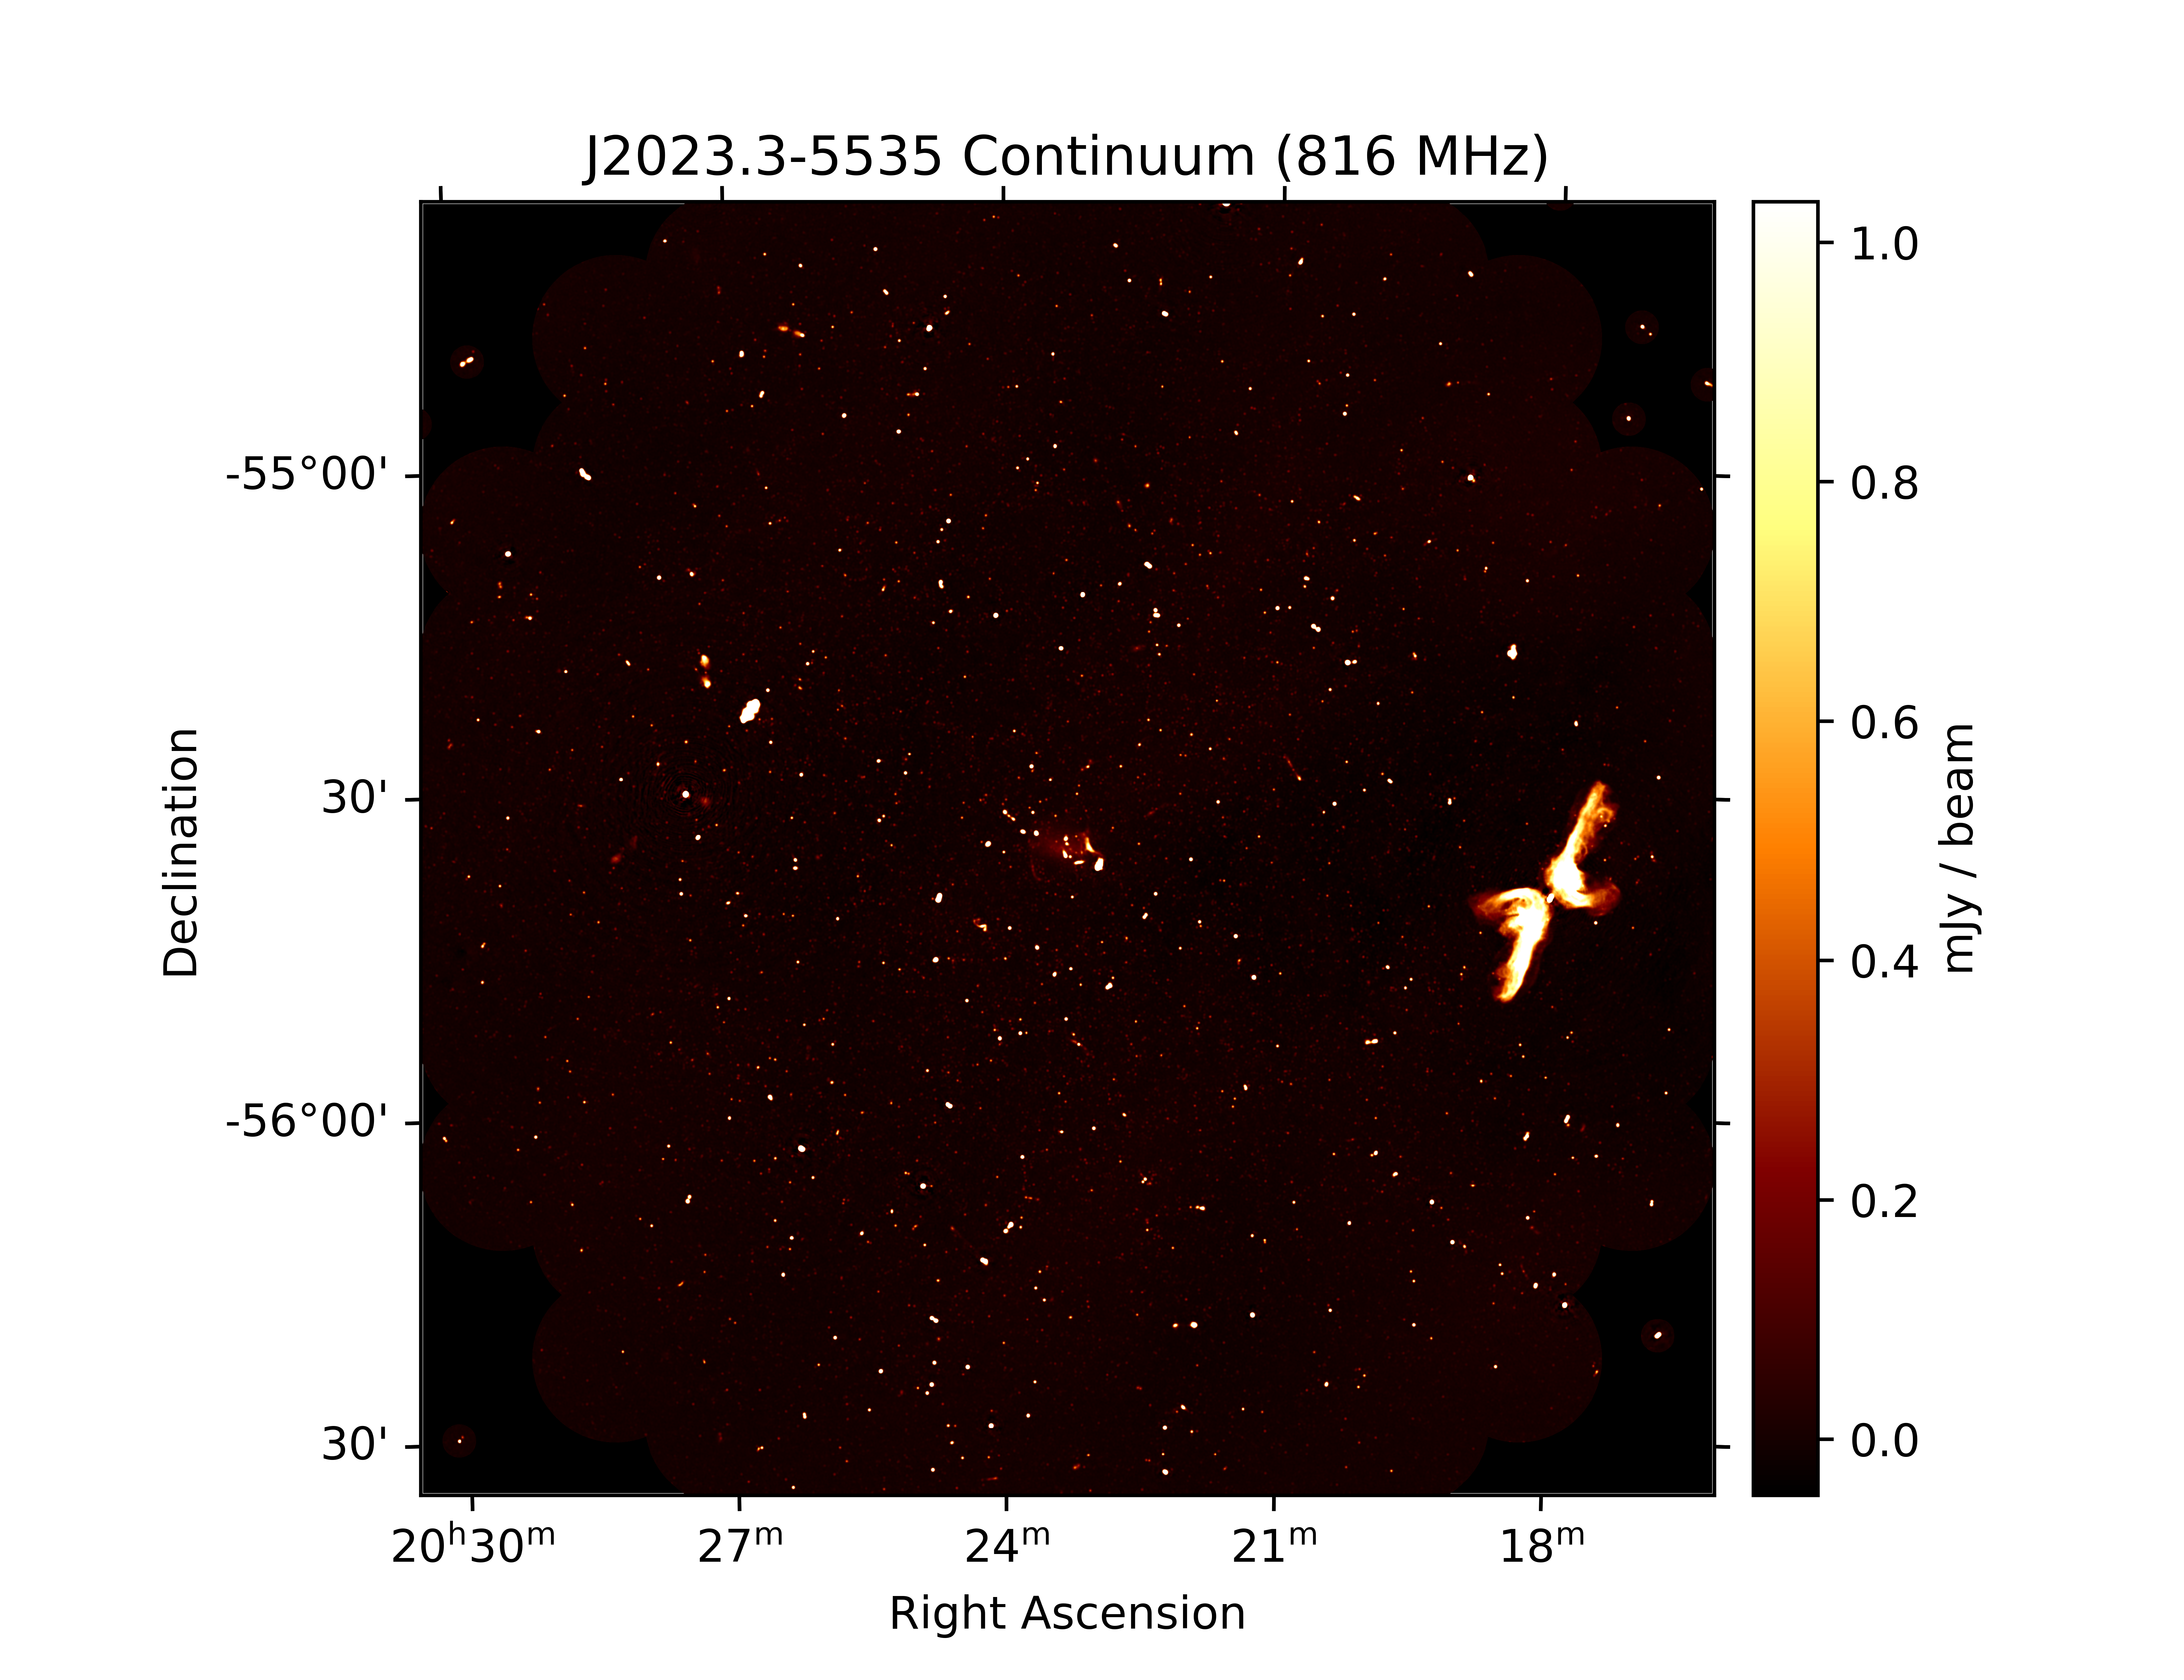
\includegraphics[width=0.5\textwidth]{MeerKAT_Image.png}
  \caption{An example UHF continuum thumbnail image produced automatically by the continuum imaging pipeline is shown above, \citep{ratcliffeSDPPipelinesOverview2021}}
  \label{fig:Meerkat_Image}
\end{figure}

This dataset is then split into eight 107 MHz intermediate frequencies \citep{ratcliffeSDPPipelinesOverview2021}.
The UV data's headers contain the number of antennas, the number of baselines, the number of channels, and the number of polarization \citep{ratcliffeSDPPipelinesOverview2021}.
In the 48-antenna Meerkat's array, short baselines dominate \citep{ratcliffeSDPPipelinesOverview2021}. This allows baseline-dependent averaging to reduce data volume \citep{ratcliffeSDPPipelinesOverview2021}.
This step reduces the data volume by about 3-4 times \citep{ratcliffeSDPPipelinesOverview2021}.

The \texttt{MFImage} task uses joint frequency deconvolution to handle wide-band effects in wide-band images \citep{ratcliffeSDPPipelinesOverview2021}. 
Normally, Meerkat uses approximately 140 circular image facets with a size of ~6 arcminutes to cover 1 degree from the phase center \citep{ratcliffeSDPPipelinesOverview2021}.
Additionally, there are facets of 1 degree that  use the SUMSS or NVSS catalogue to cover a radius of 2.5 degrees from the phase center \citep{ratcliffeSDPPipelinesOverview2021}.
These 1-degree facets are used for phenomena that are ancipiated to have a flux density greater than 5 mJy \citep{ratcliffeSDPPipelinesOverview2021}.
The facets integrate wide-band imaging effects. The frequency band is split into 10 components \citep{ratcliffeSDPPipelinesOverview2021}. 
During joint-frequency deconvolution, the brightest sources in the dataset are found and subtracted from the slices of data individualy using the CLEAN algorithm \citep{ratcliffeSDPPipelinesOverview2021}.

Self-calibration is then performed in two rounds. The first round uses CLEAN components with a flux density above 1 mJy. This yields approximately 1000 CLEAN components \citep{ratcliffeSDPPipelinesOverview2021}. 
The data are then self calibrated in a second round, using a CLEAN threshhold of 100 $\mu$Jy. The second round yields approximately 10000 CLEAN components \citep{ratcliffeSDPPipelinesOverview2021}.
After this process, the field continuum images are produced.
Lastly, the self calibrated data is converted into AIPS format \citep{ratcliffeSDPPipelinesOverview2021}.
The sky model, made up of the CLEAN components, is stored in AIPS CC format. The flux density of all the 10 frequency components are summed \citep{ratcliffeSDPPipelinesOverview2021}. The merged flux density is then fitted with a second degree polynomial over frequency and subtracted from the image \citep{ratcliffeSDPPipelinesOverview2021}.
Finally, the fully processed images are converted into FITS and PNG files and archived \citep{ratcliffeSDPPipelinesOverview2021}.

 \textbf{(3) The Spectral Pipeline:} 
The purpose of the spectral imaging pipeline is to produce high-quality spectral line images effectively \citep{ratcliffeSDPPipelinesOverview2021}. 
Spectral channels are independent of each other, and can be processed in parallel \citep{ratcliffeSDPPipelinesOverview2021}. However, the raw resulting data are recieved in time-major order, and this data structure must be transposed in channel-major order \citep{ratcliffeSDPPipelinesOverview2021}.
In order to solve this issue, a visibility writer is used. The writer stores the visibilities on a Ceph cluster \footnote{\url{https://ceph.io/en/}} with chunks each across 64 spectral channels \citep{ratcliffeSDPPipelinesOverview2021}. This choice in the chunk size is not optimized, but it does avoid issues with RAM and memory allocation \citep{ratcliffeSDPPipelinesOverview2021}.

Using CUDA \footnote{\url{https://developer.nvidia.com/cuda-zone}}, every channel then is imaged separately. The use of CUDA allows for the processing to speed up due to the usage of NVIDIA GPUs \citep{ratcliffeSDPPipelinesOverview2021}. 
The iteration over W slice in each chanel is shown in psuedo-code in Fig 4 (Fig. 1 of \citep{ratcliffeSDPPipelinesOverview2021})
 \begin{figure}[h!]
  \centering
  \includegraphics[width=0.9\textwidth]{Meerkat_Spec_pipeline.png}
  \caption{The inner cyclic algorithm used by the MeerKAT spectral line pipeline, \citep{ratcliffeSDPPipelinesOverview2021}}
  \label{fig:Spec_pipeline}
\end{figure}

The chunk system only partially solves the problem of transposing the data and further steps are necessary \citep{ratcliffeSDPPipelinesOverview2021}. The visibilities in each chunk are ordered by channel, w slice (wide-field imaging plane), and baseline. The data chunks inherently store measurements such as UVW coordinateas and parallatic angles \citep{ratcliffeSDPPipelinesOverview2021}.
At this point, conservative baseline-depedent averaging is also applied to the visibilities \citep{ratcliffeSDPPipelinesOverview2021}. The coordinates of every visibility are solved for, then visibilities with matching coordinates are merged, which is the last of the preprocessing of the visiblities \citep{ratcliffeSDPPipelinesOverview2021}.


\subsubsection{The Square Kilometre Array (SKA)}

\textbf{New text starts here, I dont know why my figure has 2 footnotes, I have compiled multiple times and I have only put one footnote:}
\section{Results}

\subsection{The Optical Data Results}

\subsubsection{The Sloan Digital Sky Survey (SDSS)}
Since 1998, the SDSS has published nineteen data releases and five generations, each with their own goals. Most recently, SDSS-IV planned to use spectroscopic surveys to detect cosmological objects \citep{ahumada16thDataRelease2020}.
The sixteenth data release is the first one that utilizies the SDSS-IV \citep{ahumada16thDataRelease2020}. While the seventeenth data release is the last one that utilizies the SDSS-IV. 
I plan to compare these two data releases.
The reason I'm not comparing the eighteenth data release is because it was mainly used to set the foundation for future SDSS-V data releases by introducing new models, functions, strategies, and more \citep{almeidaEighteenthDataRelease2023}.
The nineteenth release is also not applicable to this comparison because it is only a preview of what is achievable by the SDSS-V \citep{collaborationNineteenthDataRelease2025}
I believe it is important to compare these two data releases because they quantify the increase of data acquisition within the same generation.

\begin{figure}[h!]
  \centering
  \includegraphics[width=0.5\textwidth]{volume_incremental-dr17.png}
  \caption{A graph from the SDSS-IV \footnote{\url{https://www.sdss4.org/dr17/data_access/volume/}} website, showing the increase of data volume throughout multiple data releases}
  \label{fig:volume_incremental-dr17}
\end{figure}

According to Figure 6, it is clear that every data release has grown in terms of volume data. The first few generations increased only slightly, and the later generations increased exponentially. This is a clear example of Moore's Law. 
The sixteenth data release accounts for approximately 18.1\% of the SDSS-IV's total data, and the seventeeth data release accounts for approximately 37.7\% of the SDSS-IV's total data.
The seventeenth data release consists of over 46 million new files, which is the reason for the massive increase in data volume \citep{almeidaEighteenthDataRelease2023}. This increase in data can be summarized in four reasons \citep{almeidaEighteenthDataRelease2023}. 

The first reason is because the seventeenth data release accounts for the entirety of the APOGEE-2 survey, which had an additional 879,437 infrared spectral measurements \citep{almeidaEighteenthDataRelease2023}.
The second reason is because the MaNGA survey also completed \citep{almeidaEighteenthDataRelease2023}. The MaNGA survey released had 11273 cubes compared to the sixteenth data release's 4824 cubes \citep{almeidaEighteenthDataRelease2023}. These cubes hold 3D data, which two spacial dimensions and one wavelength dimension \citep{sdssMaNGAData2019}.
The third reason is because of the eBOSS survey \citep{almeidaEighteenthDataRelease2023}. Although the number of data is the same between the sixteenth and seventeenth data release, the seventeenth data release contains 25 value-added catalogues (VAC) that were either updates, or added \citep{almeidaEighteenthDataRelease2023}.
These VACs contain numerous amounts of processed data that astronomers then use, so each VAC accounts for a substantial portion of the seventeenth data release's total data \citep{almeidaEighteenthDataRelease2023}.
The last reason is the seventeenth data release includes all the previous SDSS data releases' data \citep{almeidaEighteenthDataRelease2023}. The data has been reprocessed with, what was at the time, the newest pipelines dedicated towards data processing \citep{almeidaEighteenthDataRelease2023}. The updated pipelines accounts for a substantial amount of new data, as more data can be derived from more effective processes \citep{almeidaEighteenthDataRelease2023}

The comparison of only two consecutive generations has shown a massive increase in data volume. This trend is likely to explode with the release of SDSS-V and its new components, which we will discuss later in the discussion section.

\subsubsection{The Rubin/Large Synoptic Survey Telescope (LSST)}

\subsection{The Radio Data Results}

\subsubsection{The MeerKAT}

\subsubsection{The Square Kilometre Array (SKA)}


\textbf{New text ends here:}

\section{Discussion}
\subsection{Open Source Policies and Transparency}

\subsubsection{The SDSS Policy}

The SDSS-IV  collaboration states that all of its software is open source under the BSD-3 license.
However, the SDSS outlines practices for users who wish to reuse or extend the SDSS software. Most importantly, proper citation of software and websites is required. 

\begin{figure}[h!]
  \centering
  \includegraphics[width=0.5\textwidth]{SDSS_Optical_Image.png}
  \caption{A spectrographical image obtained using data collected from SDSS}
  \label{fig:SDSS_Optical_Image}
\end{figure}

The SDSS has also implemented digital object identifiers (DOI) in all software code. These DOIs allow software and data to be easily identified, which is important for ownership.
The SDSS team also promotes transparency in coding by Git and SVN \footnote{\url{https://subversion.apache.org/}} to version code repositories.

Overall, the SDSS has demonstrated a strong commitment to making their data and software open source and transparent. This in turn helps the development of science, by ensuring that knowledge is accessible to all regardless of resources. 

\subsubsection{The LSST Policy}
Despite providing fully public data, the LSST has committed to open source software and a transparent pipeline. 
The LSST has declared that any source code made for data management must have an Open Source Initiative license \citep{verarubinobservatoryLSSTLicensingOverview}. 
Open source data-management software must be issued under the GNU Public license \citep{verarubi+nobservatoryLSSTLicensingOverview}. Otherwise, users are free to choose any Open Source initative approved license \citep{verarubinobservatoryLSSTLicensingOverview}. 

\subsubsection{The MeerKAT Policy}
The South African Radio Astronomy Observatory (SARAO) has expressed that MeerKAT data products must be open source with adequate acknowledgement through two steps \citep{camiloDOCUMENTDISTRIBUTION2024}. 
First and foremost, all MeerKAT data used must come from the MeerKAT ADS Library\footnote{\url{https://ui.adsabs.harvard.edu/public-libraries/wmc9yO6IQ3mUZCPx7MQRxg}} \citep{camiloDOCUMENTDISTRIBUTION2024}. 
Secondly, any publication that contains MeerKAT data, the author must state the following statement: "The MeerKAT telescope is operated by the South African Radio Astronomy Observatory, which is a facility of the National Research Foundation, an agency of the Department of Science and Innovation." \citep{camiloDOCUMENTDISTRIBUTION2024}.

Data products can be released into the MeerKAT archive by contacting the SARAO. \citep{camiloDOCUMENTDISTRIBUTION2024}. 
The SARAO has developed a help desk \footnote{\url{https://commons.datacite.org/doi.org?query=client.uid\%3Awhno.ljncxe\&resource-type=dataset}}
from which users can ask general questions \citep{camiloDOCUMENTDISTRIBUTION2024}. If users have questions on policies of the MeerKAT, they are advised to communicate them to the SARAO chief scientist \citep{camiloDOCUMENTDISTRIBUTION2024}.
There is also a SARAO Users Committee, reporting to the SARAO MD \citep{camiloDOCUMENTDISTRIBUTION2024}.

\subsubsection{The SKA Policy}

\subsection{The Rise of AI/ML in Surveys}


\lstset{
    basicstyle=\ttfamily\small,
    backgroundcolor=\color{gray!10},
    frame=single,
    breaklines=true,
    keywordstyle=\color{blue},
    commentstyle=\color{gray!70}\itshape,
    stringstyle=\color{orange},
    numbers=left,
    numberstyle=\tiny,
    stepnumber=1,
    numbersep=8pt,
    captionpos=b
}


\begin{appendices}

\section{Python Code for SDSS Data Retrieval (Figure 3)}
\label{Appendix}
\begin{lstlisting}[language=Python]
#Import relevant libraries/functions
from astroquery.sdss import SDSS
from astropy import coordinates as coords
import astropy.units as u
import matplotlib.pyplot as plt
import numpy as np

#Initalize Right Ascension and Declination
ra = 20
dec = -10

#Convert ra and dec into a SkyCoord Object
coord = coords.SkyCoord(ra, dec, unit='deg', frame = 'icrs')

#Query the SDSS System to find object given coordinates in a radius of 0.01 degrees
result = SDSS.query_region(coord,  radius=0.01*u.deg, spectro=True)
print(result)
#Retrieve the Image from found object, make into a FITS File
image = SDSS.get_images(matches=result, band=['u', 'g', 'r', 'i', 'z'])


#Retrieve hdulist from FITS file
hdulist = image[0]

#Retrieve the image data from the hdulist 
imageData = hdulist[0].data

#Log the image data in order to get rid of background
imageDataLog = np.log10(imageData) + 1e-8

#Save the header
header = hdulist[0].header


#Obtain the relevant headers

#Retrieve pixel scale numbers, divided amongst two parts for ra and dec 
CD1_1 = header['CD1_1']
CD1_2 = header['CD1_2']
CD2_1 = header['CD2_1']
CD2_2 = header['CD2_2']

#Width of image in pixels 
keyWordNAXIS1 = header['NAXIS1'] #[pixels]

#Height of image in pixels [pixels]
keyWordNAXIS2 = header['NAXIS2'] #[pixels]

#Normalize the pixel scale, then multiply by 3600 to convert units
CDELT1ArcSec = np.linalg.norm([CD1_1,CD1_2]) * 3600 #[arcsec/pixels]
CDELT2ArcSec = np.linalg.norm([CD2_1,CD2_2]) * 3600 #[arcsec/pixels]

#Set up the image
plt.xlabel("Right Ascension (arcsec)")
plt.ylabel("Declination (arcsec)")
plt.title('SDSS Logarithmic Optical Image')
vmin2 = np.percentile(imageDataLog, 85) 
vmax2 = np.percentile(imageDataLog, 98)
plt.imshow(imageDataLog, cmap='viridis', extent = (0, CDELT1ArcSec * keyWordNAXIS1, 0, CDELT2ArcSec * keyWordNAXIS2), vmin = vmin2, vmax = vmax2)
plt.colorbar()

plt.show()

\end{lstlisting}

\end{appendices}


\bibliography{references}
\bibliography{filename}

\end{document}


